\documentclass[spanish, 10pt,a4paper]{article}
\usepackage[spanish]{babel}
\usepackage[utf8]{inputenc}
\usepackage{textcomp}
\usepackage{hyperref}
\usepackage[pdftex]{graphicx}
\usepackage{epsfig}
\usepackage{amsmath}
\usepackage{hyperref}
\usepackage{amssymb}
\usepackage{color}
\usepackage{graphics}
\usepackage{amsthm}
\usepackage{subcaption}
\usepackage{caratula}
\usepackage{fancyhdr,lastpage}
\usepackage[paper=a4paper, left=1.4cm, right=1.4cm, bottom=1.4cm, top=1.4cm]{geometry}
\usepackage[table]{xcolor} % color en las matrices
\usepackage[font=small,labelfont=bf]{caption} % caption de las figuras en letra mas chica que el texto
\usepackage[ruled,vlined,linesnumbered]{algorithm2e}
\usepackage{listings}
\usepackage{float}
\usepackage{pdfpages}
\usepackage{amsfonts}
\usepackage{upgreek}


\color{black}

%%%PAGE LAYOUT%%%
\topmargin = -1.2cm
\voffset = 0cm
\hoffset = 0em
\textwidth = 48em
\textheight = 164 ex
\oddsidemargin = 0.5 em
\parindent = 2 em
\parskip = 3 pt
\footskip = 7ex
\headheight = 20pt
\pagestyle{fancy}
\lhead{IS1 - Trabajo Pr\'actico 1} % cambia la parte izquierda del encabezado
\renewcommand{\sectionmark}[1]{\markboth{#1}{}} % cambia la parte derecha del encabezado
\rfoot{\thepage}
\cfoot{}
\numberwithin{equation}{section} %sets equation numbers <chapter>.<section>.<subsection>.<index>

\newcommand{\figurewidth}{1\textwidth}

\newcommand{\tuple}[1]{\ensuremath{\left \langle #1 \right \rangle }}
\newcommand{\Ode}[1]{\small{$\mathcal{O}(#1)$}}


%El siguiente paquete permite escribir la caratula facilmente
\hypersetup{
  pdftitle={ IS1 - TP1 },
  colorlinks,
  citecolor=black,
  filecolor=black,
  linkcolor=black,
  urlcolor=black 
}

\materia{Ingeniería de Software I}

\titulo{Trabajo Práctico 1}

\subtitulo{Informe y diagramas.}

\grupo{Grupo 2}

\integrante{De Sousa Bispo, Germán}{359/12}{germandesousa@gmail.com}
\integrante{Fernandez, Esteban}{691/12}{esteban.pmf@gmail.com}
\integrante{Kodelia, Erika Natasha}{767/11}{erikankodelia@gmail.com}
\integrante{Mongi Badia, Martín}{422/13}{martinmongi@gmail.com}
\integrante{Sánchez Cano, Gonzalo}{}{xeneize__86@hotmail.com}
\integrante{Wright, Carolina}{876/12}{wright.carolina@gmail.com}

 
\begin{document}
{ \oddsidemargin = 2em
	\headheight = -20pt
	\maketitle
}
	\tableofcontents
	\newpage
\section{Introducción}
	El Ministro de Gobierno quiere modificar el Sistema Electoral Nacional y para ello propone instalar en las escuelas máquinas emisoras de sufragios. Junto con esta incorporación se deberá modificar el Sistema del Centro de Cómputos Nacional para que pueda operar con las máquinas.

	El formato de la votación no presenta cambios, es decir, al igual que en el sistema de boletas que se venía utilizando se permitirá votar por categorías o votar en blanco. 
	
	Además se busca proveer todos los mecanimos necesarios para asegurar el derecho de voto a todos los Electores. Se considerarán las necesidades de los no videntes y personas con movilidad reducida. 

\subsection{Alcance del software}

\newpage
\section{Describiendo el problema}

\subsection{Presunciones de dominio}
\begin{itemize}
\item Las escuelas tiene las instalaciones necesarias para el acceso de discapacitados
\item Los presidentes de mesa están capacitados para ayudar durante el voto ante dudas de uso del sistema
\item Hay un Encargado de las máquinas por zona
\item Ante falla en máquina de voto, el Encargado de las máquinas solucionará el problema en un tiempo acotado
\item La cantidad de boletas provistas a cada escuela se corresponde, como mínimo, a la cantidad de Electores
\item Los electores votan en el horario establecido
\item Las escuelas tienen cable de red o WIFI para poder comunicarse con los servidores locales y nacionales
\item El día anterior a la votación se realiza la instalación de las máquinas 
\item En caso de un Elector ciego y sordo, el mismo podrá votar con la asesoría de un tutor o bien presentar un certificado de incapacidad.
\end{itemize}

\subsection{Requerimientos}
\begin{itemize}
\item El Elector puede votar una única vez
\item Para poder, votar el Elector debe aparecer en el Padrón de la escuela
\item El voto se realiza de a un Elector por vez
\item Manejar correctamente la situación en la que el Elector presenta alguna discapacidad o es no vidente
\item El Presidente de mesa y los Fiscales no utilizan la máquina durante la elección
\item La máquina permite realizar el voto si la boleta fue insertada
\item Las máquinas tienen conexión a internet
\item Las máquinas se actualizan el día anterior
\item La batería de las máquinas inicia el día con la carga completa
\end{itemize}

\subsection{Principales alternativas}

\section{Casos hipotéticos}

Agregamos unos casos hipotéticos en los cuales aparecerán los agentes y objetivos de una manera más definida a fin de entender mejor el sistema que planteamos.

\subsection{Curso de una votación estándar}
	El Elector averigua el lugar en donde le corresponde votar y el día de la votación concurre a la escuela que le fue asignada. Una vez ahí se presenta y anuncia en la mesa. El Presidente de Mesa y Fiscales comprueban los datos, le entregan un ticket y le permiten dirigirse a la máquina emisora de sufragio. 

	Para poder realizar el voto, el Elector ingresa en ticket único en la máquina y a partir de allí comenzará a elegir los candidatos. Una vez que navegó por las categorías o eligió lista completa podrá  realizar un clic en "finalizar votación". A continuación se imprimirá, en el ticket antes ingresado, los datos de los candidatos elegidos. El Elector podrá confirmar que sus elecciones se corresponden con lo presente en el ticket pasando el mismo por el lector que se encuentra en la máquina. Como la información esta correcta procede al paso siguiente.

	Con el ticket impreso en mano se presenta nuevamente en la mesa y lo ingresa en la urna.	
	
\subsection{Incorrecta elección de candidatos}
	Siguiendo el ejemplo anterior, el Elector realiza la misma votación. Una vez terminada, decide confirmar su voto haciendo uso del lector. Allí se da cuenta que los datos que el ingresó no son lo que quería, es decir, su intención de voto no se ve reflejada en el ticket. Luego, se acerca a la mesa y explica lo sucedido. El Presidente de Mesa rompe el ticket con los datos incorrectos y le entrega uno nuevo. El Elector vuelve a repetir el proceso y finaliza como el caso anterior. 

\subsection{Incorrecto funcionamiento de la máquina}
	Durante el proceso de votación al Elector se le presenta un problema: la máquina no funciona correctamente. Luego de dar conocimiento de lo sucedido al Presidente de Mesa, éste último se comunicará con el Encargado de Máquinas quien concurrirá en un tiempo razonable a reparar la misma. 

	Mientras y hasta que se solucione el inconveniente, la mesa se moverá para hacer uso de las máquinas extras que se encuentran en la planta baja  (mismas en las que votarán los Electores con discapacidad). En las mismas,  el Presidente de Mesa seleccionará la mesa que corresponde y el Elector podrá votar con normalidad.

\subsection{Elector discapacitado}
	Como las escuelas cuentan con las instalaciones necesarias para el acceso de cualquier persona, el Elector con discapacidad puede ingresar al establecimiento sin problemas. Una vez allí pueden ocurrir dos escenarios: su mesa se encuentra a su alcance (esta en planta baja) o no.
	
	Si se encuentra en el primer caso, realiza el voto de manera estándar sin complicaciones. 
	
	Si se encuentra en el segundo se avisará en la mesa que le corresponde y el Presidente bajará con la urna hacia el cuarto especialmente preparado para esta situación.	Este cuarto se encuentra en planta baja por lo que el Elector podrá acceder cómodamente. Antes de que el Elector pueda acercase a la máquina, el Presidente de Mesa ingresará el número de mesa correspondiente en la misma. Esto es necesario dado que el conteo de votos se realiza primero por mesa, luego por escuela y por último en la totalidad. Entonces, como este cuarto es para uso de discapacitados que pueden pertenecer a diferentes mesas, la máquina que allí se encuentra sumará votos de distintas mesas si no se indica lo contrario. A continuación el Elector procede a votar normalmente.

\subsection{Elector no vidente}

	En este caso, cuando el Elector se presenta en la mesa se le entregan unos auriculares. Éstos servirán para guiarlo durante el proceso de votación indicando los movimientos a realizar y la ubicación de los candidatos en la pantalla.

\section{Métodos de autenticación}

	Nuestro sistema de votación electrónico, deberá contar con algún método a través del cual asegurarse que no se emitan sufragios ilegítimos (por ejemplo, que un elector vote dos veces o que vote alguien que no estaba en el padrón). Para esto, en nuestro diagrama de objetivos tenemos un o-refinamiento, en el cual planteamos varias formas de autenticación: 

	\begin{itemize}

		\item El Presidente de Mesa le otorga una boleta al Elector, la cual la Máquina imprime y devuelve al Elector. Luego, este deposita la boleta ya impresa en la urna. Este método tiene la ventaja de ser más económico, ya que la máquina de votación no tiene otros requerimientos de hardware que la impresora. Sin embargo, es imposible para el conteo interno de la máquina comprobar que no haya habido fraude, por lo tanto los conteos provisorios podrían ser inexactos, ya que dependen exclusivamente del conteo por software.
		\item El Presidente de Mesa le otorga una boleta al Elector, el cual la coloca en la Máquina. Luego, esta le pide que se autentique. Dicha autenticación se lleva a cabo de a través de métodos biométricos, a través del cual se verifica la identidad del elector, que pertenezca al padrón de la Mesa y que no haya votado previamente. Si es autenticado, la Máquina le permite sufragiar, imprime la boleta y se la devuelve al Elector. Este método tiene la ventaja de que el fraude es improbable. Sin embargo, tiene el costo agregado de que cada Máquina debe contar con un sensor biométrico del tipo elegido. Hay varios tipos de autenticación biométrica, que varían en seguridad y costo de implementación. Para nuestro método consideraremos el que autentica a través de las huellas dactilares, aprovechando que PJN ya cuenta con esa base de datos, y que provee un nivel aceptable de seguridad y costo.
	\end{itemize}


\newpage
\section{Vistas}
\subsection{Diagrama de Contexto}

\begin{figure}[H]
  \centering
  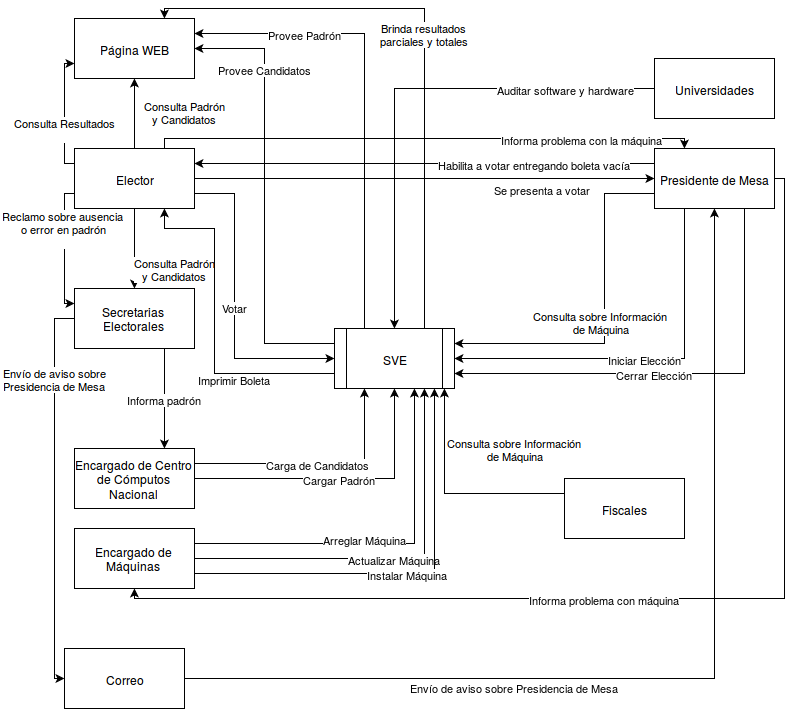
\includegraphics[scale=0.50]{pdf/DiagramaDeContexto}
  \caption{Diagrama de contexto}
  \label{fig:DiagramaDeContexto}
\end{figure}

\begin{itemize}
\item La relación \textit{Se presenta a votar} entre el \textit{Elector} y el \textit{Presidente de Mesa} engloba, además del caso estándar, que el \textit{Elector} sea discapacitado, por lo que dando el aviso al \textit{Presidente de Mesa}, para que el último baje la urna, seleccione el número de mesa en la máquina de votación y entregue la boleta con la que el \textit{Elector} votará (englobado en la relación \textit{Habilita a votar entregando boleta vacía}).
\item La relación \textit{Votar} entre el \textit{Elector} y \textit{SVE} implica que el \textit{Elector} realice todo el proceso de votación que debe realizar la máquina. Esto implica la inserción de la boleta en la máquina, la selección de los candidatos a votar, la confirmación de los datos si es deseado y depositar la boleta impresa en la urna.
\item La relación \textit{Consulta sobre información de Máquina} establecida entre el \textit{Presidente de Mesa} y \textit{SVE}, así como también entre \textit{Fiscales} y \textit{SVE} contienen la consulta sobre los candidatos que ofrece la máquina y, una vez cerrados los comicios, los resultados parciales y totales, ya sea de la máquina como de la votación.
\item La relación \textit{Actualizar Máquina} dada entre el \textit{SVE} y el \textit{Encargado de Máquinas} representa la descarga de los datos que se utilizarán para los comicios (candidatos, listas, etc). De esta forma, se evitan errores por carga manual.
\end{itemize}

%\subsection{Diagrama de Objetivos}
\clearpage
% \begin{figure}[H]
%   \centering
%   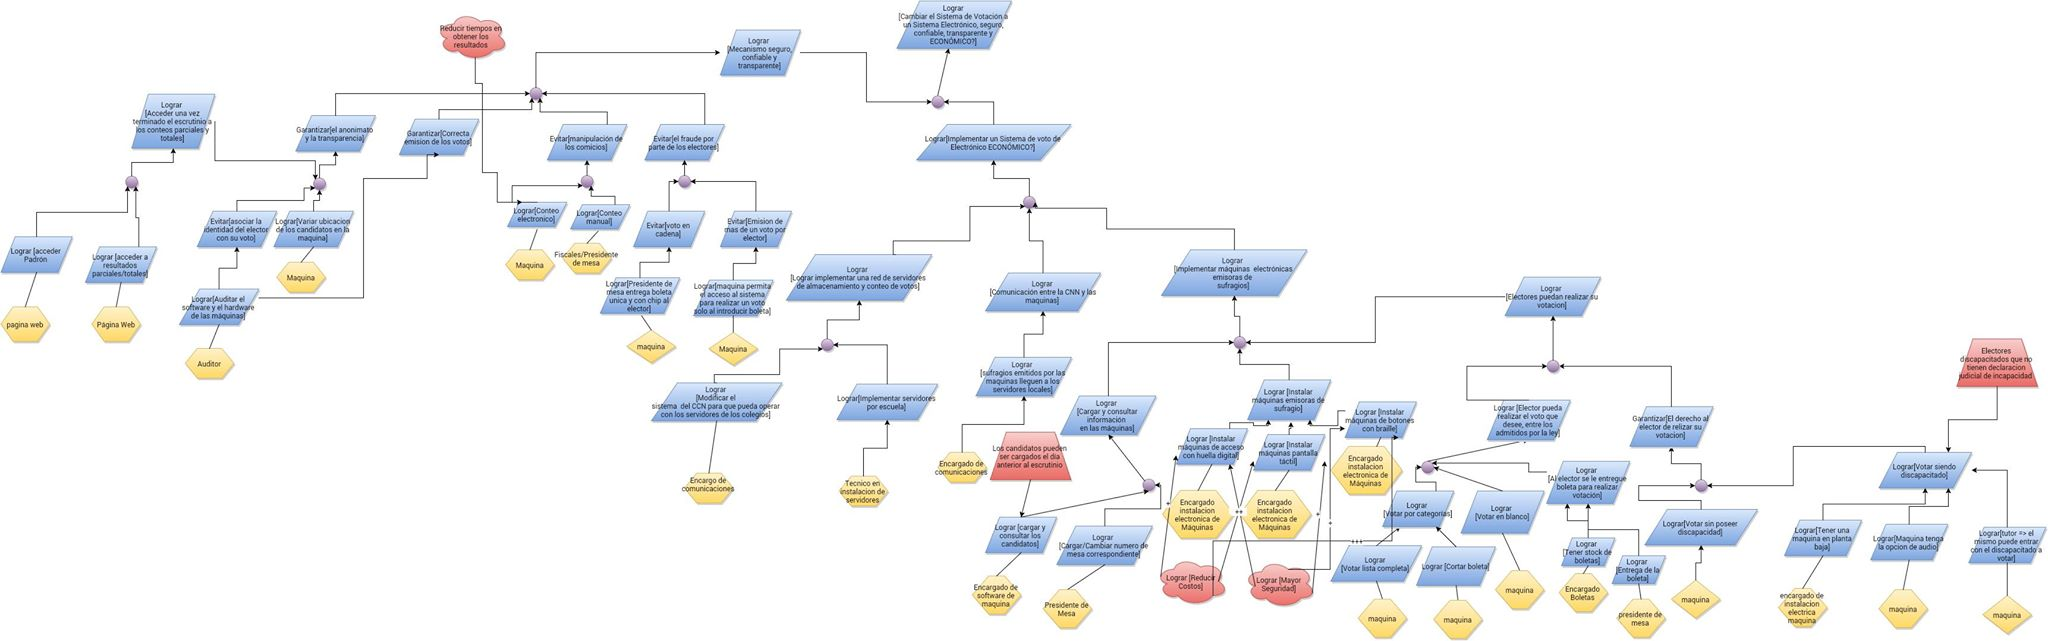
\includegraphics[scale=0.50]{pdf/Diagrama de objetivos.jpg}
%   \caption{Diagrama de contexto}
%   \label{fig:DiagramaDeContexto}
% \end{figure}
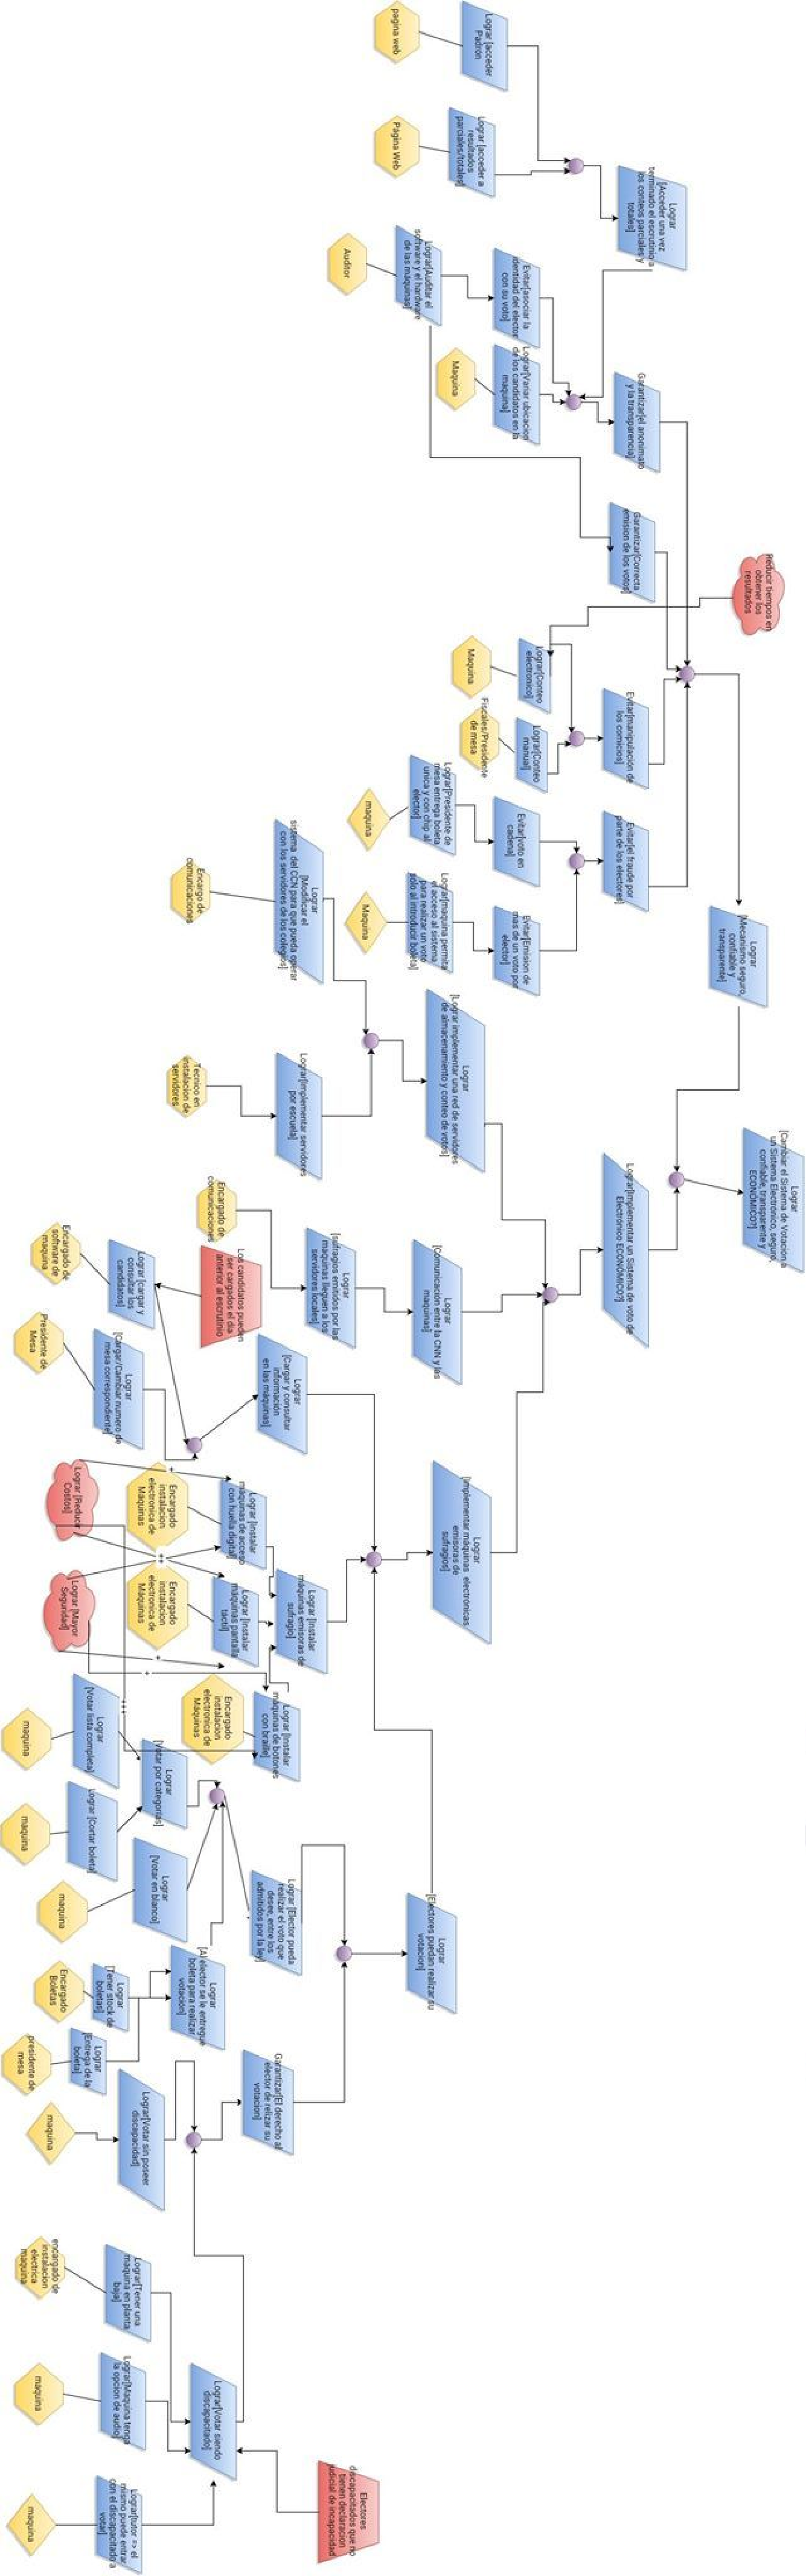
\includepdf{pdf/DiagramaDeObjetivos.pdf}
\newpage

\section{Conclusión}
	\newpage
	%~ \newpage
	%~ \bibliographystyle{plain}
	%~ \clearpage
	%~ \bibliography{bibliography}
	%~ \addcontentsline{toc}{section}{Referencias}

\newpage
\section{Listado de cosas que queremos lograr - PRE ENTREGA}

Dada la característica de pre-entrega, y para que se entienda cuáles son las cosas que queremos lograr para resolver el problema, agregamos el listado de factores que consideramos importantes y cómo nos imaginamos que el sistema funcionará: 

\begin{itemize}
\item Para el caso de cargos asignados en proporción a los votos conseguidos (diputados por ejemplo) conversión proporcional de votos siguiendo el Método D Hont.
\item Asignar presidente de Mesa para todas las mesas de todos los lugares de votación del país
\item Registro y consulta de Resultados parciales y totales, una vez cerrado los comicios
\item Lograr cambiar sistema de votación.. máquinas emisoras de sufragios
\item Lograr un mecanismo seguro y transparente
\item Lograr modificar el sistema del Centro de Cómputos Nacional
\item Instalar máquinas emisoras de sufragios, una por mesa.
\item Lograr cargar y consultar el Padrón según el lugar de votación
\item Cargar y consultar los Candidatos
\item Se puedan cargar los Candidatos previamente al día del escrutinio
\item Garantizar que todos los electores puedan ejercer su derecho.
\item Permitir votar por categorías  / cortar boleta
\item Permitir votar en blanco
\item Permitir votar lista completa
\item Cada Presidente de Mesa puede dar inicio a la elección el día de los comicios, habilitando a los electores que figuren en el padrón de la mesa correspondiente.
\item El Elector elija candidatos con la garantía irrestricta de que va a poder ejercer su derecho a votar en plenitud.
\item Se preste asistencia en el momento del escrutinio (es decir, en el conteo de los votos).
\item Se imprimirá una boleta con la votación realizada.
\item Se tendrán pantallas táctiles. Alternativas: pantalla tipo cajero con botones con número en braille, pantalla táctil con braille.
\item Garantizar el derecho a los no videntes o con movilidad reducida. 
\item Para los que tienen movilidad reducida se situarán máquinas para votar en planta baja en el cual el presidente de mesa ingresará el número de mesa correspondiente a la que debería haber votado.
\item En caso de los ciegos estará la posibilidad mediante audio con auriculares para mantener el secreto del voto.
\item En el caso de ruptura de una máquina, se utilizará el mismo medio que los discapacitados hasta que la misma se arregle.
\item Minimizar o mitigar los errores.
\item Minimizar errores humanos.
\item Al final de proceso de votación se le mostrará al elector todas sus elecciones.
\item Minimizar errores técnicos (plantear diferentes métodos de conteo transmisión y carga de datos)
\item Contar con una estrategia de sincronización para la transmisión de datos de todas las máquinas distribuidas por el país.
\item Auditar los comicios antes y después de la elección y de participar en su administración y en el escrutinio, el fiscal general.
\item La boleta será depositada en una urna. 
\item El conteo de los votos se hará automáticamente. (para lograr que estén los resultados a las dos horas)
\item El voto será enviado directo a un servidor del colegio. Luego estos votos serán enviados a su vez a un servidor central en el Centro de Computo Nacional. 
\item El conteo de los votos se hará, además, manualmente con las boletas de la urna para que los fiscales puedan corroborar los resultados o con máquina que cuenta boletas
\item Los Fiscales designados por los partidos puedan ejercer su derecho a controlar los comicios.
\item Garantizar una competencia electoral igualitaria.
\item La posición de los candidatos en la pantalla debe variar para cada Elector. (ambos lados)
\item Los datos quedarán guardados en la máquina de manera digital.
\item Evitar el fraude.
\item Evitar la manipulación de los comicios.
\item Evitar fraudes tradicionales como el voto cadena.(varía el formato la boleta o huella digital)
\item Garantizar el anonimato y la transparencia
\item Evitar asociar la identidad del Elector con su voto.
\item Auditar el software y el hardware de las máquinas. Que el código sea validado por universidades previamente para asegurar que no se usa la información del elector.
\item Máquinas con batería que puedan durar todo el día. Igualmente conectadas.
\item Reducir el costo en comparación al sistema tradicional. 
\item Reducir costos en materia de fiscalización y en la impresión de boletas partidarias.(papel ecológico)
\item Evitar el robo de boletas en el cuarto oscuro. 
\item Usuario presidente o fiscal que pueda leer información de la máquina (conteo de votos una vez cerrada la mesa, candidatos, abrir mesa, cerrar mesa, etc) (con tarjeta identificatoria, huella digital,  o password???????? ) 
\item Permite votar si se le inserta una boleta dada por el presidente de mesa para poder votar. 
\end{itemize}


\end{document}